\documentclass[12pt,a4paper]{article}

% ── Packages ──────────────────────────────────────────────────────────────────
\usepackage[margin=1in]{geometry}
\usepackage{amsmath, amssymb, amsthm}
\usepackage{graphicx}
\usepackage{float}
\usepackage{caption}
\usepackage{subcaption}
\usepackage{hyperref}
\usepackage{booktabs}
\usepackage{xcolor}
\usepackage{listings}
\usepackage{enumitem}
\usepackage{fancyhdr}
\usepackage{titlesec}
\usepackage{parskip}
\usepackage{array}
\usepackage{multirow}
\usepackage{tikz}
\usetikzlibrary{arrows.meta, shapes.geometric, positioning}

% ── Colors ────────────────────────────────────────────────────────────────────
\definecolor{accent}{RGB}{0, 102, 204}
\definecolor{codebg}{RGB}{245, 245, 245}
\definecolor{kw}{RGB}{0, 0, 180}
\definecolor{str}{RGB}{0, 128, 0}
\definecolor{cmt}{RGB}{128, 128, 128}

% ── Code listings ──────────────────────────────────────────────────────────────
\lstset{
  backgroundcolor=\color{codebg},
  basicstyle=\ttfamily\small,
  keywordstyle=\color{kw}\bfseries,
  stringstyle=\color{str},
  commentstyle=\color{cmt}\itshape,
  breaklines=true,
  frame=single,
  framerule=0.4pt,
  rulecolor=\color{gray!40},
  numbers=left,
  numberstyle=\tiny\color{gray},
  numbersep=6pt,
  xleftmargin=12pt,
  language=Python,
  showstringspaces=false,
  tabsize=4,
  captionpos=b,
}

% ── Header / Footer ───────────────────────────────────────────────────────────
\pagestyle{fancy}
\fancyhf{}
\rhead{\textcolor{gray}{\small SMAI Assignment 3}}
\lhead{\textcolor{gray}{\small Personalised Indian Recommender (T14.1)}}
\rfoot{\thepage}

% ── Section styling ───────────────────────────────────────────────────────────
\titleformat{\section}{\large\bfseries\color{accent}}{{\thesection}}{1em}{}[\titlerule]
\titleformat{\subsection}{\normalsize\bfseries}{{\thesubsection}}{1em}{}

% ── Hyperlinks ────────────────────────────────────────────────────────────────
\hypersetup{colorlinks=true, linkcolor=accent, urlcolor=accent, citecolor=accent}

% ─────────────────────────────────────────────────────────────────────────────
\begin{document}

% ── Title Page ────────────────────────────────────────────────────────────────
\begin{titlepage}
  \centering
  \vspace*{2cm}
  {\LARGE\bfseries SMAI — Assignment 3\par}
  \vspace{0.5cm}
  {\Large\color{accent} T14.1 — Cook with What I Have\par}
  {\large Personalised Indian Recipe Recommender\par}
  \vspace{1.5cm}
  \rule{\linewidth}{0.4pt}\\[0.8cm]

  % ── Team details — fill in roll numbers and emails ─────────────────────────
  \begin{tabular}{ll}
    \textbf{Name} & Achyutananda Sahoo \\
    \textbf{Roll Number} & \texttt{[ROLL NUMBER]} \\
    \textbf{Email} & \texttt{achu23022002@gmail.com} \\[0.8em]
    % Add teammates below if applicable:
    % \textbf{Name} & Teammate 2 \\
    % \textbf{Roll Number} & \texttt{[ROLL NUMBER]} \\
    % \textbf{Email} & \texttt{[EMAIL]} \\
  \end{tabular}\\[0.8cm]
  \rule{\linewidth}{0.4pt}\\[0.8cm]

  {\large International Institute of Information Technology, Hyderabad\par}
  \vspace{0.4cm}
  {\large Statistical Methods in AI\par}
  \vspace{0.4cm}
  {\large May 2026\par}
  \vspace{2cm}

  \begin{abstract}
    \normalsize
    We present a content-based recipe recommendation system for Indian cuisine.
    Given a natural-language query (a list of available ingredients or a dish name),
    the system returns a ranked list of relevant recipes from a dataset of 6{,}865
    Indian recipes. The pipeline combines sentence-transformer embeddings with
    cosine similarity retrieval, accelerated by a FAISS index, and augmented with
    a keyword-overlap scoring term to improve ingredient-level precision. A
    Streamlit web application exposes the system with filters, a favourites page,
    and developer tooling for live tuning of scoring parameters.
  \end{abstract}
\end{titlepage}

\tableofcontents
\newpage

% ─────────────────────────────────────────────────────────────────────────────
\section{Introduction}
% ─────────────────────────────────────────────────────────────────────────────

Recommendation systems are among the most widely deployed machine-learning
techniques in industry. This project implements a real, small-scale recommender
for an Indian-flavour domain following the T14.1 variant specification: a
\emph{``Cook with What I Have''} recipe assistant.

The core challenge is to rank a corpus of recipes by relevance to a free-text
query without any user interaction history or explicit ratings. We therefore
adopt a \textbf{content-based retrieval} approach, encoding both queries and
recipes as dense semantic vectors and retrieving by vector similarity.

\subsection{Objectives}
\begin{itemize}[leftmargin=2em]
  \item Build a no-training recommendation pipeline using sentence embeddings.
  \item Improve ingredient-level precision via hybrid keyword--semantic scoring.
  \item Accelerate retrieval using a FAISS vector index.
  \item Expose all functionality through an interactive Streamlit application.
\end{itemize}

% ─────────────────────────────────────────────────────────────────────────────
\section{Dataset}
% ─────────────────────────────────────────────────────────────────────────────

We use the \textbf{Indian Food Dataset} \cite{kaggle_dataset}, available on
Kaggle (\texttt{kanishk307/6000-indian-food-recipes-dataset}).

\subsection{Statistics}

\begin{table}[H]
  \centering
  \begin{tabular}{ll}
    \toprule
    Property & Value \\
    \midrule
    Total recipes (raw) & 6{,}871 \\
    After cleaning (drop null) & 6{,}865 \\
    Cuisine categories & 25+ \\
    Diet categories & 7 \\
    Course categories & 12 \\
    Cook-time range & 5 – 1{,}440 min \\
    \bottomrule
  \end{tabular}
  \caption{Dataset summary statistics}
\end{table}

\subsection{Key Columns}

\begin{table}[H]
  \centering
  \begin{tabular}{ll}
    \toprule
    Column & Description \\
    \midrule
    \texttt{TranslatedRecipeName} & English recipe name \\
    \texttt{TranslatedIngredients} & Comma-separated ingredient list (English) \\
    \texttt{Cuisine} & e.g.\ North Indian, South Indian, Gujarati \\
    \texttt{Diet} & e.g.\ Vegetarian, Non-Vegetarian, Vegan \\
    \texttt{Course} & e.g.\ Main Course, Snack, Dessert \\
    \texttt{TotalTimeInMins} & Prep + cook time \\
    \bottomrule
  \end{tabular}
  \caption{Relevant dataset columns}
\end{table}

\subsection{Preprocessing}

Each recipe is reduced to a single \texttt{combined\_text} string:

\begin{lstlisting}[caption={Building combined\_text}]
df["combined_text"] = (
    df["TranslatedRecipeName"] + " "
    + df["TranslatedIngredients"] + " "
    + df["Cuisine"] + " "
    + df["Diet"] + " "
    + df["Course"]
)
\end{lstlisting}

This concatenation ensures that the embedding model can attend to all
semantically relevant fields simultaneously.

% ─────────────────────────────────────────────────────────────────────────────
\section{System Architecture}
% ─────────────────────────────────────────────────────────────────────────────

\begin{figure}[H]
  \centering
  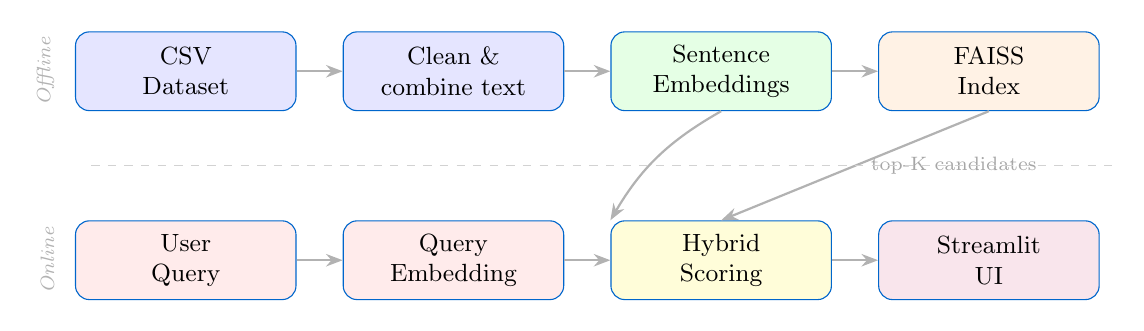
\begin{tikzpicture}[
    box/.style={
      rectangle, draw=accent, rounded corners=5pt,
      minimum width=2.8cm, minimum height=1cm,
      text centered, font=\small\linespread{1}\selectfont,
      align=center
    },
    arr/.style={-{Stealth[length=6pt]}, thick, color=gray!60},
    lbl/.style={font=\scriptsize, color=gray!80, midway, above=2pt}
  ]

  % ── Row 1: offline / build-time pipeline ───────────────────────
  \node[box, fill=blue!10]   (csv)   at (0,   0) {CSV\\Dataset};
  \node[box, fill=blue!10]   (clean) at (3.4, 0) {Clean \&\\combine text};
  \node[box, fill=green!10]  (embed) at (6.8, 0) {Sentence\\Embeddings};
  \node[box, fill=orange!10] (faiss) at (10.2,0) {FAISS\\Index};

  \draw[arr] (csv)   -- (clean) node[lbl]{};
  \draw[arr] (clean) -- (embed) node[lbl]{};
  \draw[arr] (embed) -- (faiss) node[lbl]{};

  % ── Row 2: query-time pipeline ─────────────────────────────────
  \node[box, fill=red!8]     (query) at (0,  -2.4) {User\\Query};
  \node[box, fill=red!8]     (qemb)  at (3.4,-2.4) {Query\\Embedding};
  \node[box, fill=yellow!15] (rank)  at (6.8,-2.4) {Hybrid\\Scoring};
  \node[box, fill=purple!10] (ui)    at (10.2,-2.4){Streamlit\\UI};

  \draw[arr] (query) -- (qemb)  node[lbl]{};
  \draw[arr] (qemb)  -- (rank)  node[lbl]{};
  \draw[arr] (rank)  -- (ui)    node[lbl]{};

  % ── Cross arrows: index + embeddings feed into ranking ─────────
  \draw[arr] (faiss.south) -- (rank.north)
    node[font=\scriptsize, color=gray!70, midway, right=2pt]{top-K candidates};
  \draw[arr] (embed.south) to[bend right=15] (rank.north west);

  % ── Row labels ─────────────────────────────────────────────────
  \node[font=\scriptsize\itshape, color=gray!60, left=4pt] at (csv.west)
    {\rotatebox{90}{Offline}};
  \node[font=\scriptsize\itshape, color=gray!60, left=4pt] at (query.west)
    {\rotatebox{90}{Online}};

  % ── Dashed separator ───────────────────────────────────────────
  \draw[dashed, color=gray!35, line width=0.5pt]
    (-1.2, -1.2) -- (11.8, -1.2);

  \end{tikzpicture}
  \caption{End-to-end recommendation pipeline. \textit{Offline}: embeddings and
  FAISS index are built once and cached. \textit{Online}: each user query is
  embedded, retrieved via FAISS, re-ranked with hybrid scoring, and rendered.}
\end{figure}

% ─────────────────────────────────────────────────────────────────────────────
\section{Methodology}
% ─────────────────────────────────────────────────────────────────────────────

\subsection{Step 1 — Sentence Embeddings}

We use the pre-trained \textbf{\texttt{all-MiniLM-L6-v2}} model from the
\texttt{sentence-transformers} library \cite{sbert}. It maps any text string to
a dense vector in $\mathbb{R}^{384}$:

\begin{equation}
  \mathbf{e}_i = f_\theta(\text{combined\_text}_i) \in \mathbb{R}^{384}
\end{equation}

where $f_\theta$ is the transformer encoder with fixed (pre-trained) weights
$\theta$. No fine-tuning is performed — the model is used purely at inference
time.

\medskip
\noindent The full corpus produces an embedding matrix:
\begin{equation}
  E = \begin{bmatrix} \mathbf{e}_1^\top \\ \mathbf{e}_2^\top \\ \vdots \\
  \mathbf{e}_N^\top \end{bmatrix} \in \mathbb{R}^{N \times 384}, \quad N = 6{,}865
\end{equation}

\subsection{Step 2 — Cosine Similarity Retrieval}

Given a user query $q$, we embed it with the same model:
$\mathbf{q} = f_\theta(q) \in \mathbb{R}^{384}$.

The relevance of recipe $i$ to query $q$ is measured by \textbf{cosine similarity}:

\begin{equation}
  \text{sim}_{\cos}(\mathbf{q}, \mathbf{e}_i)
  = \frac{\mathbf{q} \cdot \mathbf{e}_i}{\|\mathbf{q}\|\,\|\mathbf{e}_i\|}
  = \frac{\sum_{k=1}^{384} q_k \, e_{ik}}
         {\sqrt{\sum_k q_k^2}\;\sqrt{\sum_k e_{ik}^2}}
  \in [-1,\, 1]
\end{equation}

Cosine similarity measures the \emph{angle} between vectors, making it
length-invariant — a recipe described in one sentence scores the same as one
described in ten sentences if their directions match.

The top-$K$ results are selected by:
\begin{equation}
  \mathcal{R}_K = \underset{i \in [N]}{\operatorname{top-K}}\;
  \text{sim}_{\cos}(\mathbf{q}, \mathbf{e}_i)
\end{equation}

\subsubsection{Limitation of Pure Semantic Search}

When a query contains specific ingredients such as \textit{``fish, onion''},
the embedding for ``onion'' dominates because onion appears in $\sim$80\% of
Indian recipes, pulling the query vector toward generic onion dishes and
diluting the signal from ``fish''. This motivates the hybrid scoring approach
described in Section~\ref{sec:hybrid}.

\subsection{Step 3 — FAISS Accelerated Retrieval}
\label{sec:faiss}

Computing $\text{sim}_{\cos}(\mathbf{q}, \mathbf{e}_i)$ for all $N$ recipes is
$O(N \cdot d)$ per query. For large corpora this becomes a bottleneck.
\textbf{FAISS} (Facebook AI Similarity Search) \cite{faiss} provides
CPU-optimised exact and approximate nearest-neighbour search.

\subsubsection{L2 Normalisation Trick}

For unit-norm vectors, the inner product equals cosine similarity:
\begin{equation}
  \hat{\mathbf{e}}_i = \frac{\mathbf{e}_i}{\|\mathbf{e}_i\|}, \quad
  \hat{\mathbf{q}} = \frac{\mathbf{q}}{\|\mathbf{q}\|}
  \implies
  \hat{\mathbf{q}} \cdot \hat{\mathbf{e}}_i = \text{sim}_{\cos}(\mathbf{q}, \mathbf{e}_i)
\end{equation}

We therefore L2-normalise all vectors before adding to the FAISS index, allowing
us to use the fast \texttt{IndexFlatIP} (Inner Product) index.

\subsubsection{Index Types Used}

\begin{table}[H]
  \centering
  \begin{tabular}{llll}
    \toprule
    Index & Search type & Time complexity & Use case \\
    \midrule
    \texttt{IndexFlatIP}  & Exact    & $O(N)$           & $N < 500$K \\
    \texttt{IndexIVFFlat} & Approximate & $O(\sqrt{N})$ & $N > 100$K \\
    \bottomrule
  \end{tabular}
  \caption{FAISS index types compared}
\end{table}

\subsubsection{IVF — Inverted File Index}

\texttt{IndexIVFFlat} partitions the vector space into $n_{\text{list}}$
Voronoi cells using $k$-means clustering. At query time, only the
$n_{\text{probe}}$ nearest cells are searched:

\begin{equation}
  n_{\text{list}} = 4\sqrt{N} \approx 331, \qquad
  n_{\text{probe}} = \left\lfloor \frac{n_{\text{list}}}{10} \right\rfloor = 33
\end{equation}

\noindent \textbf{Benchmark results} (50 repeated queries, $N = 6{,}865$):

\begin{table}[H]
  \centering
  \begin{tabular}{lccc}
    \toprule
    Method & Search type & Time per query & Recall@10 \\
    \midrule
    sklearn cosine & Exact & $\sim$18 ms & 100\% \\
    FAISS Flat     & Exact & $\sim$1 ms  & 100\% \\
    FAISS IVF      & Approximate & $\sim$0.17 ms & $\sim$94\% \\
    \bottomrule
  \end{tabular}
  \caption{Search speed and accuracy comparison}
\end{table}

\subsection{Step 4 — Hybrid Scoring}
\label{sec:hybrid}

To address the ingredient dilution problem, we augment cosine similarity with
a \textbf{keyword overlap score}.

\subsubsection{Keyword Overlap Score}

Let $K = \{k_1, k_2, \ldots, k_m\}$ be the set of keywords extracted from the
query (tokens of length $> 2$), and let $I_i$ be the ingredient text of
recipe $i$. The keyword overlap score is:

\begin{equation}
  \text{kw}(K, I_i) = \frac{|\{k \in K : k \subseteq I_i\}|}{|K|}
  \in [0, 1]
\end{equation}

This fraction equals 0 if no query keyword appears in the recipe's
ingredients, and 1 if all keywords are present.

\subsubsection{Blending — Convex Combination}

The final score is a convex combination of both signals, controlled by a
weight $w \in [0, 1]$:

\begin{equation}
  \boxed{
    \text{score}(q, i) = (1 - w)\cdot\text{sim}_{\cos}(\mathbf{q}, \mathbf{e}_i)
    + w \cdot \text{kw}(K, I_i)
  }
\end{equation}

Since both terms lie in $[0, 1]$ and $w + (1-w) = 1$, the blended score is
also in $[0, 1]$ — this is a valid \emph{convex combination}.

\begin{table}[H]
  \centering
  \begin{tabular}{lll}
    \toprule
    $w$ & Behaviour & Best for \\
    \midrule
    0.0 & Pure cosine similarity & Vague queries: ``something spicy'' \\
    0.35 & Hybrid (default) & Balanced ingredient + meaning \\
    1.0 & Pure keyword overlap & Exact ingredient matching \\
    \bottomrule
  \end{tabular}
  \caption{Effect of keyword weight $w$}
\end{table}

\subsubsection{Effect on Example Query}

For the query \textit{``fish, onion''}:

\begin{itemize}
  \item At $w=0$ (pure cosine): top results are generic onion dishes; no fish.
  \item At $w=0.35$ (default): fish recipes rank at top-1.
  \item At $w=1.0$ (pure keyword): only recipes with both exact words surface.
\end{itemize}

% ── Screenshot placeholder ────────────────────────────────────────────────────
\begin{figure}[H]
  \centering
  \includegraphics[width=1\textwidth]{image.png}
  \caption{Ranked Cards - query : "fish, onion"}
\end{figure}


% ─────────────────────────────────────────────────────────────────────────────
\section{Streamlit Application}
% ─────────────────────────────────────────────────────────────────────────────

The system is exposed through a Streamlit web application with two navigable
pages.

\subsection{Recommender Page}

\begin{itemize}
  \item \textbf{Query input}: free-text box or one-click ingredient chips.
  \item \textbf{Sidebar filters}: cuisine, diet, course, max cook time, number of results.
  \item \textbf{Ranked cards}: each card shows recipe name, match score, cuisine,
        diet, cook time, and an expandable ingredient list with \textbf{query
        keywords highlighted} in orange.
  \item \textbf{Why?} caption: explains why each recipe was recommended —
        lists matched ingredients, diet tag, and cook time.
  \item \textbf{Save to Favourites}: toggle button per recipe.
\end{itemize}

% ── Screenshot placeholder ────────────────────────────────────────────────────
\begin{figure}[H]
  \centering
  \includegraphics[width=1\textwidth]{home.png}
  \caption{Recommender tab}
\end{figure}

\begin{figure}[H]
  \centering
  \includegraphics[width=1\textwidth]{ranked_cards.png}
  \caption{Ranked Cards - query : "fish, onion"}
\end{figure}


\subsection{Favourites Page}

Saved recipes persist for the session and are accessible via a dedicated tab.
Each saved card includes cuisine metadata and a Remove button. A ``Clear all''
button wipes the list.

% ── Screenshot placeholder ────────────────────────────────────────────────────
\begin{figure}[H]
  \centering
  \fbox{\begin{minipage}{0.85\textwidth}\centering\vspace{3cm}
    \textit{[Screenshot: Favourites tab showing saved recipe cards]}
  \vspace{3cm}\end{minipage}}
  \caption{Favourites tab}
\end{figure}

\subsection{Dev Tools Panel}

A toggle in the top-right corner reveals the developer panel:

\begin{itemize}
  \item \textbf{Search method}: switch between brute-force cosine and FAISS index.
  \item \textbf{Keyword boost toggle}: enable/disable the hybrid scoring term.
  \item \textbf{Keyword weight slider}: tune $w$ from 0.0 to 1.0 in real time.
  \item \textbf{Dev metrics banner}: shows search method, recipes searched,
        query time (ms), and active keyword weight.
\end{itemize}

% ── Screenshot placeholder ────────────────────────────────────────────────────
\begin{figure}[H]
  \centering
  \includegraphics[width=0.35\textwidth]{dev_tools.png}
  \caption{Recommender tab}
\end{figure}

\section{Repository Structure}
% ─────────────────────────────────────────────────────────────────────────────

\begin{verbatim}
Assignment-3/
├── Dataset/
│   └── IndianFoodDatasetCSV.csv
├── recommendation_system/
│   ├── main.py                      # Streamlit app
│   ├── walkthrough.ipynb            # Step-by-step pipeline explanation
│   ├── faiss_walkthrough.ipynb      # FAISS index deep-dive
│   ├── hybrid_scoring_walkthrough.ipynb  # Hybrid scoring math
│   └── recipe_index.faiss           # Saved FAISS index
└── report/
    └── report.tex                   # This document
\end{verbatim}

% ─────────────────────────────────────────────────────────────────────────────
\section{Conclusion}
% ─────────────────────────────────────────────────────────────────────────────

We built a functional content-based recipe recommendation system for Indian
cuisine. The key contributions are:

\begin{enumerate}
  \item A \textbf{no-training} semantic retrieval pipeline using
        \texttt{all-MiniLM-L6-v2} embeddings and cosine similarity.
  \item A \textbf{FAISS-accelerated} index reducing query time from $\sim$18 ms
        to $<$1 ms for exact search.
  \item A \textbf{hybrid scoring} formula that blends semantic similarity with
        keyword overlap, controlled by a tunable weight $w$, significantly
        improving ingredient-level precision.
  \item A \textbf{Streamlit application} with multi-page navigation,
        real-time parameter tuning via dev tools, keyword highlighting in
        ingredients, and a persistent favourites page.
\end{enumerate}

Future work could integrate ChromaDB for persistent embedding storage,
add BM25 as a third retrieval signal, and collect implicit user feedback
(clicks, saves) for personalised re-ranking.

% ─────────────────────────────────────────────────────────────────────────────
\begin{thebibliography}{9}

\bibitem{kaggle_dataset}
  Kanishk307,
  \textit{6000 Indian Food Recipes Dataset},
  Kaggle, 2022.
  \url{https://www.kaggle.com/datasets/kanishk307/6000-indian-food-recipes-dataset}

\bibitem{sbert}
  N.\ Reimers and I.\ Gurevych,
  \textit{Sentence-BERT: Sentence Embeddings using Siamese BERT-Networks},
  EMNLP 2019.
  \url{https://arxiv.org/abs/1908.10084}

\bibitem{faiss}
  J.\ Johnson, M.\ Douze, and H.\ Jégou,
  \textit{Billion-scale similarity search with GPUs},
  IEEE Transactions on Big Data, 2019.
  \url{https://arxiv.org/abs/1702.08734}

\bibitem{miniLM}
  W.\ Wang et al.,
  \textit{MiniLM: Deep Self-Attention Distillation for Task-Agnostic
  Compression of Pre-Trained Transformers},
  NeurIPS 2020.

\end{thebibliography}

\end{document}
